% !TEX encoding = UTF-8 Unicode 
% !TEX root = praca.tex

\section{Cross-platform mobile development}\label{chap:cross_mobile_dev}

As the term suggests, cross-platform or multi-platform frameworks enable to create applications that can be installed on different platforms, and consequently reach a larger user base. There are many solutions available in the market, which all offer support for a narrow or wide subset of existing platforms. Therefore, applications may be published as, e.g., mobile apps (Android, iOS), web apps, desktop apps (Windows, macOS, Linux) or even embedded apps. The number of operating systems tends to increase under the principle of ``write once, run everywhere'' followed by frameworks' creators \cite{comparison_technologies_multiplatform}.

The main advantage of cross-platform development over native development is in line with its primary goal, which is the ability to create and maintain a single codebase, no matter the number of target platforms. Moreover, as described in the chapter \ref{chap:native}, Android operating system suffers from high level of fragmentation which can be addressed with cross-platform framework as well. Being able to operate on a single codebase results in the development costs decrease. Implementation is more time-efficient without the need to build multiple projects. This remains true for post-release support in the form of updating versions and handling bugs or change requests. Cross-platform approach is also lighter on resources, requiring just a single development team, which additionally removes possible collaboration issues between teams that can occur in native approach. In the past, it would be assumed it is easier to gather an experienced team for native development, however currently the most popular multi-platform frameworks are mature enough to have created active communities with high level of know-how \cite{approach_to_assess_performance_case_study,comparison_perf_looks_flutter_native,comp_analysis_hybrid_frameworks}.

There are differences between available cross-platform frameworks, especially in the context of
architecture or rendering and compilation method. They will be described in the following chapters. Essentially, most of them require a middle layer that connects the app with the system and translates the commands to be natively called. This is considered to be a possible root of performance decrease \cite{appdynamics_mobile_app_performance}. And although a single workspace is used during development and testing, in order to publish the final application to different app stores (e.g. Google Play Store, App Store), there must be performed a build for each target platform to acquire separate app bundles that can then be uploaded \cite{comp_study_hybrid}.

As explained in the previous chapter, different operating systems usually have different guidelines provided when it comes to user interface (UI) design. This might become an issue depending on design assumptions. Considering the user's point of view, there are three approaches to UI implementation. Firstly, the app appearance may be identical regardless of the platform it runs on. In this case, the platform-specific conventions may not be fulfilled and only when implemented correctly it will not cause user experience decrease. Secondly, the app may have a completely system-compliant look and feel. In this case, the issue may be raised as to how efficient it is to implement disjointed layouts in the cross-platform solution compared to switching to the native approach. Finally, there is an intermediate approach which assumes that most of the app elements are shared between platforms, but there are some that are platform-specific, e.g., popups, action buttons \cite{cross_platform_ux,baseline_cross_platform}.

\begin{figure}[h]
    \centering
    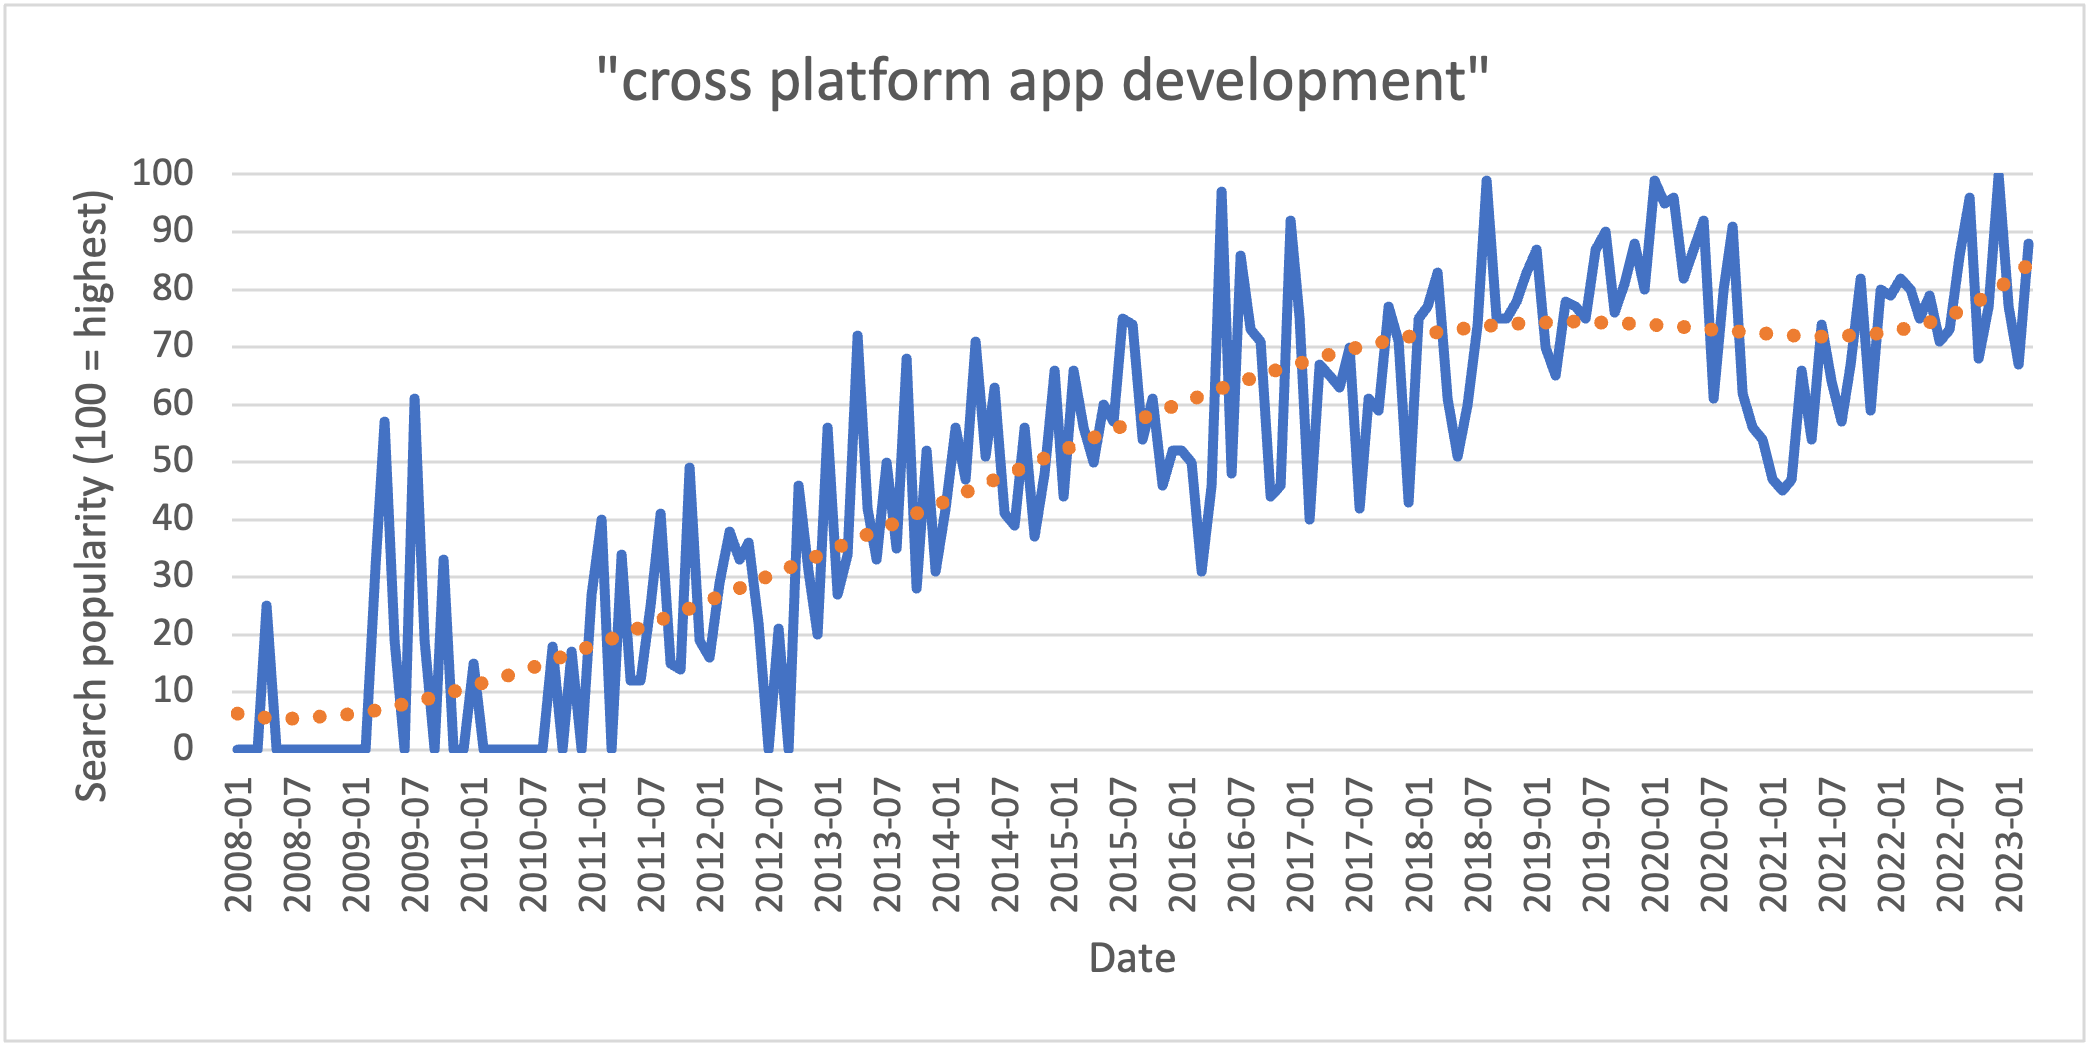
\includegraphics[width=\textwidth]{img/google_trends_cross_platform}
    \caption{Google Trends search popularity of cross-platform app development (Source: Own work based on \cite{trends_cross_platform})}
    \label{fig:trends_cross_platform}
\end{figure}

Despite the existing assumption that cross-platform frameworks might produce applications suffering from performance decrease, their popularity significantly grew during the past couple of years. The Figure \ref{fig:trends_cross_platform} shows the Google search popularity for the phrase ``cross platform app development''. The upward trend is clearly visible, which depicts the big interest in the topic amongst online users. Apache Cordova and Xamarin are examples of multi-platform frameworks which were the most popular in the beginning, however more recent solutions have already surpassed them. In Figure \ref{fig:trends_comparison} the rapid rise of Flutter and React Native can be observed as well as the ongoing importance of Ionic. These three frameworks are different from each other but still share the fact that they gather big user groups. For that reason, they have been selected to undergo a review and performance analysis inline with the goal of this thesis.

\begin{figure}[h]
    \centering
    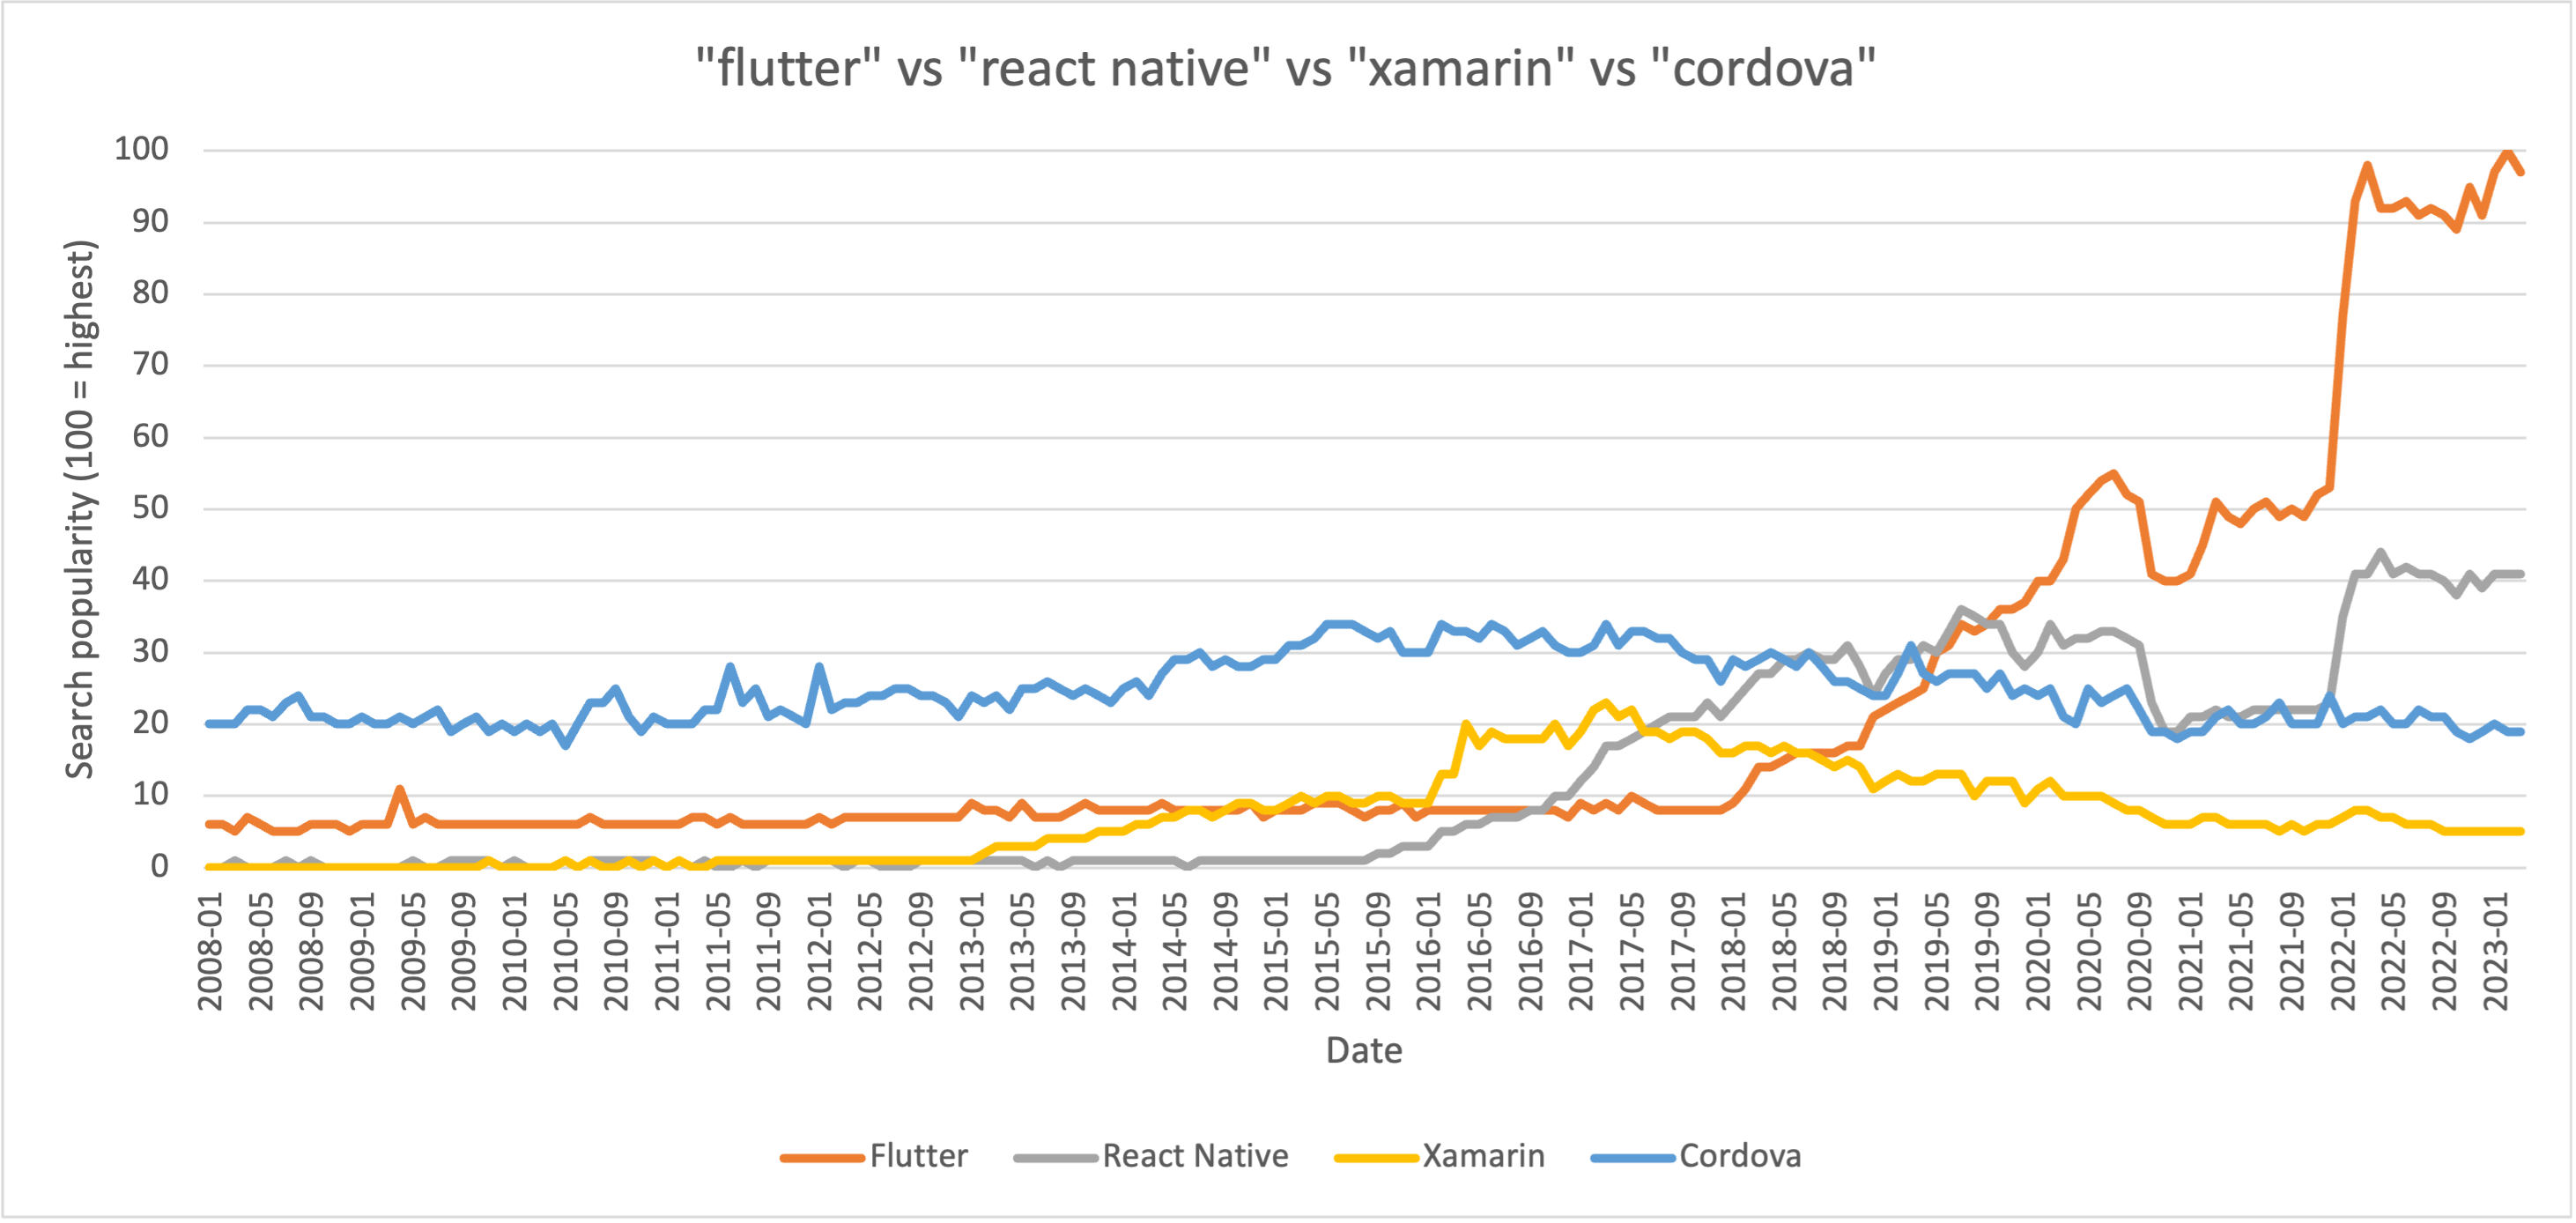
\includegraphics[width=\textwidth]{img/google_trends_comparison}
    \caption{Google Trends search popularity of selected cross-platform frameworks (Source: Own work based on \cite{trends_comparison})}
    \label{fig:trends_comparison}
\end{figure}

\subsection{Cross-platform development approaches}\label{chap:cross_platform_approaches}

Multiple types of cross-platform solutions can be distinguished. The most commonly present in the scientific literature are the following: hybrid, interpreted, cross-compiled, and Progressive Web Apps (PWAs). Native mobile development may provide better connection with native components and services compared to some of the types mentioned above. This may become the cause of lower performance.

\subsubsection*{Hybrid approach}

The term \emph{cross-platform} tends to be used interchangeably with \emph{hybrid} which technically is incorrect as these are not necessarily synonyms. The hybrid approach to cross-platform development assumes a merge of native and web applications. Typically, the web app is created with the use of web solutions, e.g. HyperText Markup Language (HTML), Cascading Style Sheets (CSS) and JavaScript (JS) which then runs inside a web view component provided by the native app, allowing to publish the end-product in regular app stores. Usually, there is a bridge enabling the usage of device native features which are out-of-scope for JS API. Figure \ref{fig:hybrid_architecture} shows the overall architecture of a hybrid application. One of the drawbacks is that the access to native components is not possible while building the user interface, which makes it more difficult to mimic the native look and feel for the user. The hybrid approach may provide a lower performance for the bigger projects because the application is executed by the browser engine and the bridge may cause overhead \cite{survey_taxonomy_cross_platform,comparison_technologies_multiplatform,cross_platform_development_study_rn_flutter,eval_rn_flutter,comp_analysis_hybrid_frameworks}.

\begin{figure}[h]
	\centering
	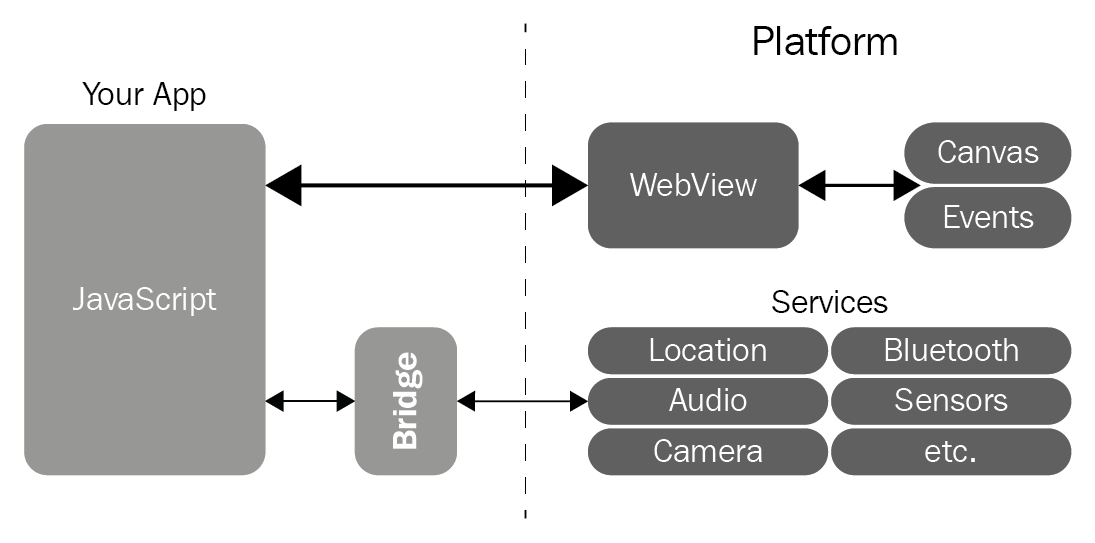
\includegraphics[width=.64\textwidth]{img/hybrid}
	\caption{Hybrid app architecture (Source: \cite{karim_flutter_different})}
	\label{fig:hybrid_architecture}
\end{figure}

\subsubsection*{Interpreted approach}

Similarly to the hybrid approach, web technologies are the primary component of the interpreted approach. The key difference between them is that interpreted apps do not use the web view. Instead, there is an interpreter involved which translates the web elements into native components that can be rendered directly in the operating system. Figure \ref{fig:interpreted_architecture} shows the overall architecture of an interpreted application. In the context of accessing the native features, there is again a bridge applied. The main advantage over the hybrid approach is the guaranteed native appearance and behavior \cite{survey_taxonomy_cross_platform,eval_rn_flutter}.

\begin{figure}[h]
	\centering
	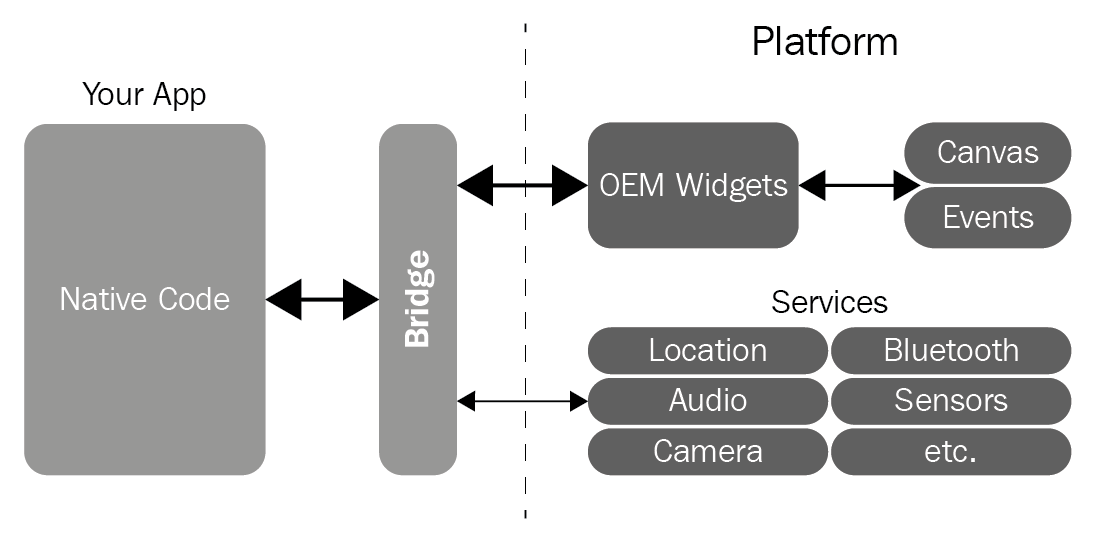
\includegraphics[width=.64\textwidth]{img/interpreted}
	\caption{Interpreted app architecture (Source: \cite{karim_flutter_different})}
	\label{fig:interpreted_architecture}
\end{figure}

\subsubsection*{Cross-compiled approach}

The cross-compiled approach introduces significant changes compared to the previously mentioned solutions. There are no additional layers between the app and the underlying operating system. The Software Development Kit enables the usage of native features and components. A cross-compiled framework uses a programming language of choice which is compiled to native byte code specific to the platform it runs on. Out of the three described approaches, this one should provide the best user experience and performance, thus gaining a lot of popularity.  \cite{survey_taxonomy_cross_platform,comparison_technologies_multiplatform,cross_platform_development_study_rn_flutter,eval_rn_flutter}.

\begin{figure}[h]
	\centering
	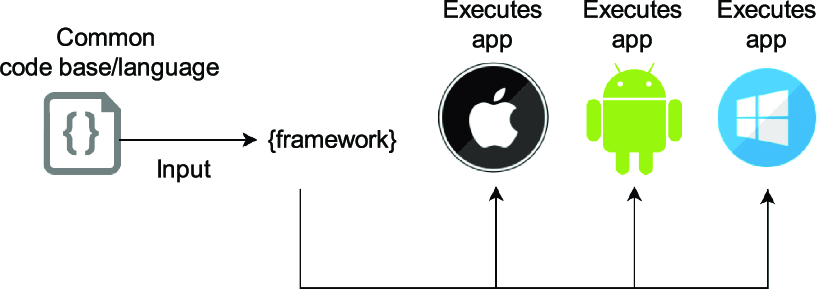
\includegraphics[width=.63\textwidth]{img/cross_compiled}
	\caption{Cross-compiled approach workflow (Source: \cite{survey_taxonomy_cross_platform})}
	\label{fig:cross_compiled_workflow}
\end{figure}

\subsubsection*{Progressive Web Apps}

Progressive Web App (PWA) is a web application that allows the user to install it on a mobile device as if it was a native app. The installation process differs because native apps are downloaded from the app store, while PWAs can be downloaded per request upon the user's visit using a web browser. In order for the web app to acquire the abilities of PWAs, they must fulfill some technical requirements, mainly the implementation of Service Workers and app manifest file. The Service Worker provides some important functions such as the control of data flow (determining whether a web server or locally cached content should be used to complete a request, see Figure \ref{fig:pwa_architecture}). PWA runs in the browser with some features hidden, e.g. address bar, which results in the appearance indistinguishable from native apps. The disadvantage of PWAs is the fact that they cannot provide full support for native components because they are limited by browser APIs. Furthermore, there is a compatibility issue as iOS 11.3 is the minimal compatible version to enable PWA installation.
\cite{survey_taxonomy_cross_platform,comparison_technologies_multiplatform,eval_rn_flutter}.

\begin{figure}[h]
	\centering
	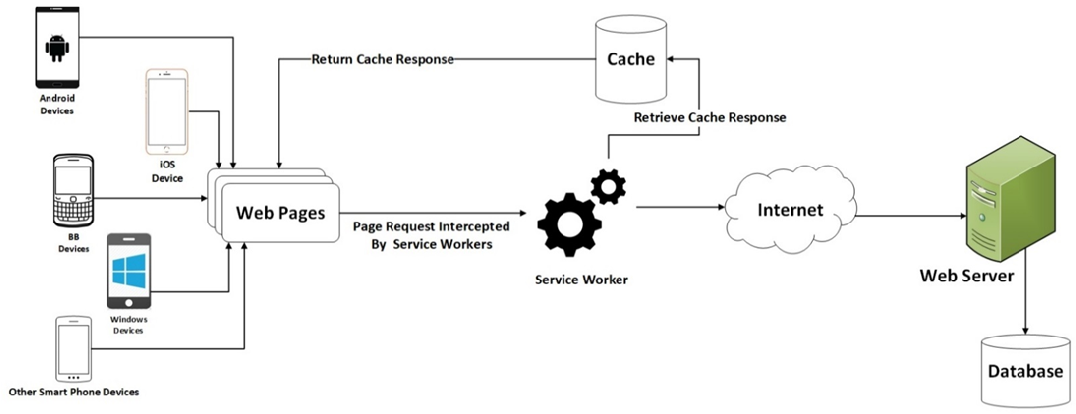
\includegraphics[width=\textwidth]{img/pwa}
	\caption{Progressive Web App architecture (Source: \cite{dawning_pwa})}
	\label{fig:pwa_architecture}
\end{figure}

\subsection{Flutter}
Flutter is a cross-platform framework belonging to the cross-compiled approach described above. It supports all the most common platforms: mobile (Android, iOS), web, desktop (Windows, macOS, Linux) and embedded. It utilizes a dedicated programming language, Dart. Being released by Google in 2017, it is a relatively recent solution. Even though, it has gathered a lot of traction in a short time, which resulted in its broad application across different segments of the market. Popular exemplary applications developed using Flutter are: Google Pay, eBay, Alibaba, BMW, Toyota and PUBG MOBILE \cite{flutter_showcase,flutter_docs_architecture}.

\subsubsection*{Architecture}

\begin{figure}[h]
    \centering
    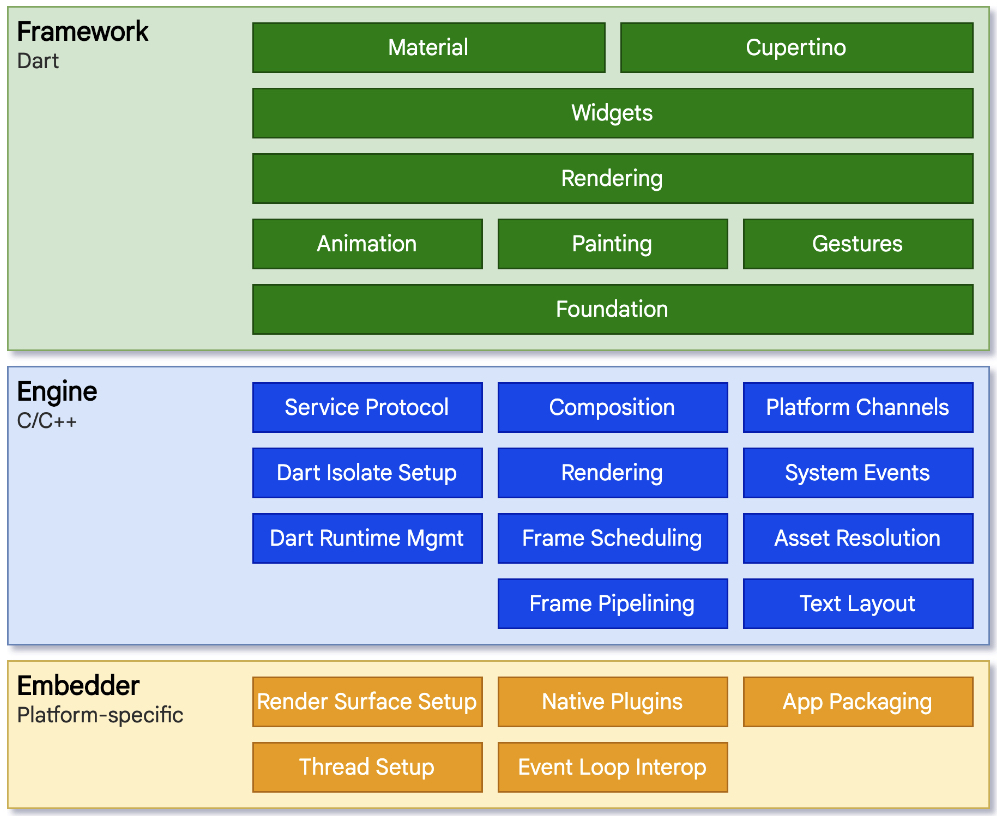
\includegraphics[width=.77\textwidth]{img/flutter_architecture}
    \caption{Flutter architecture (Source: \cite{flutter_docs_architecture})}
    \label{fig:flutter_architecture}
\end{figure}

Flutter consists of three primary layers (libraries) that are completely autonomous, as shown in Figure \ref{fig:flutter_architecture}. This makes it highly modular, with the possibility to substitute any layer by hand.

\emph{Embedder} layer is placed at the very bottom to directly interact with the operating system in order to manage surface rendering, input methods, event loop and native plugins. It is platform-specific therefore is implemented with appropriate programming languages for each platform, e.g. Java, C++, Objective-C or Objective-C++ \cite{flutter_docs_architecture}.

\emph{Engine} is the most significant layer which provides the ``low-level implementation of Flutter's core API'', meaning runtime management, platform channels, text layout, scene composition, rendering, and more. Flutter engine compiles source code to platform-specific byte code therefore there is no need for an external intermediate layer allowing communication with the underlying operating system to access any native features, such as JavaScript bridge in case of hybrid and interpreted frameworks. This provides a big advantage from the perspective of achievable performance. Moreover, from the point of view of developers, debugging is more complex with JS bridge because in order to fix any runtime errors they must be retraced through the bridge first \cite{flutter_docs_architecture,windmill_flutter_in_action}.

\emph{Engine} is also where the graphics aspect is contained. Since the very first release, Flutter has been using Skia as its graphics engine. As stated above, Flutter translates the source code to byte code instead of using an intermediate layer which would use the source code to determine native components, in the contrast to interpreted cross-platform solutions. Therefore, the byte code itself is passed directly to Skia for rendering. Importantly, a Skia copy is included in the \emph{Engine} layer in order to allow the latest version to be used even on devices with older operating system version. Moreover, this enables the app to look the same even on older devices, which would not be otherwise possible. Nonetheless, there have been some performance issues reported, especially by iOS-targeting developers. For that reason, Google has begun working on a new graphics engine for Flutter. Recently (May 2023), it was announced that the new engine, \emph{Impeller}, became enabled by default for iOS applications and is available for testing for Android. It is supposed to improve performance and eliminate jank problems.
\cite{flutter_docs_architecture,flutter_impeller,kosinski_flutter_vs_rn_vs_qt}.

The final layer, \emph{Framework}, is the interface for developers. It contains all the components required for writing applications, such as widgets, animations, Material and Cupertino libraries, etc. \cite{flutter_docs_architecture}.

\subsubsection*{Web support}

\begin{figure}[h]
    \centering
    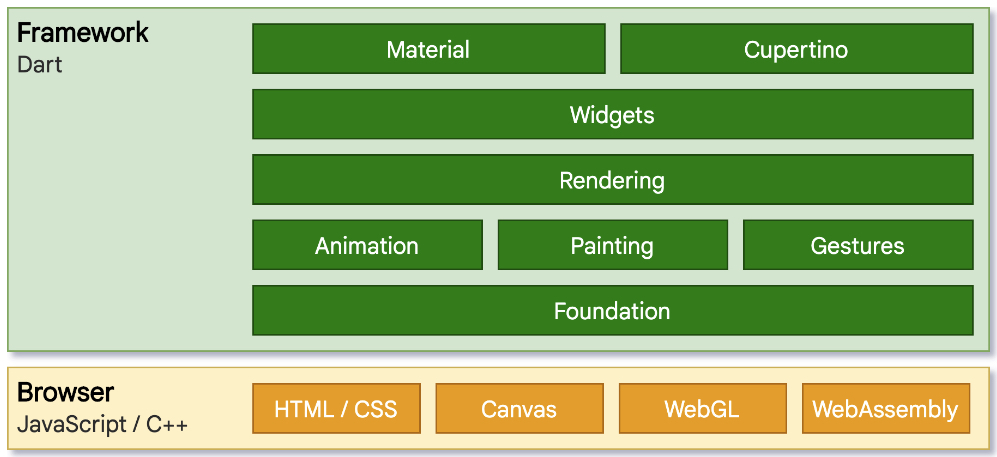
\includegraphics[width=.77\textwidth]{img/flutter_web_architecture}
    \caption{Flutter web-adapted architecture (Source: \cite{flutter_docs_architecture})}
    \label{fig:flutter_web_architecture}
\end{figure}

In order to support web, for such builds the Flutter's engine is specifically adapted to include the standard browser APIs (see Figure \ref{fig:flutter_web_architecture}). From the rendering perspective, there are two possible methods: HTML+CSS+Canvas+SVG or CanvasKit. The former minimizes the download size, while the latter usually offers better performance.

\subsubsection*{Rendering}

\begin{figure}[h]
    \centering
    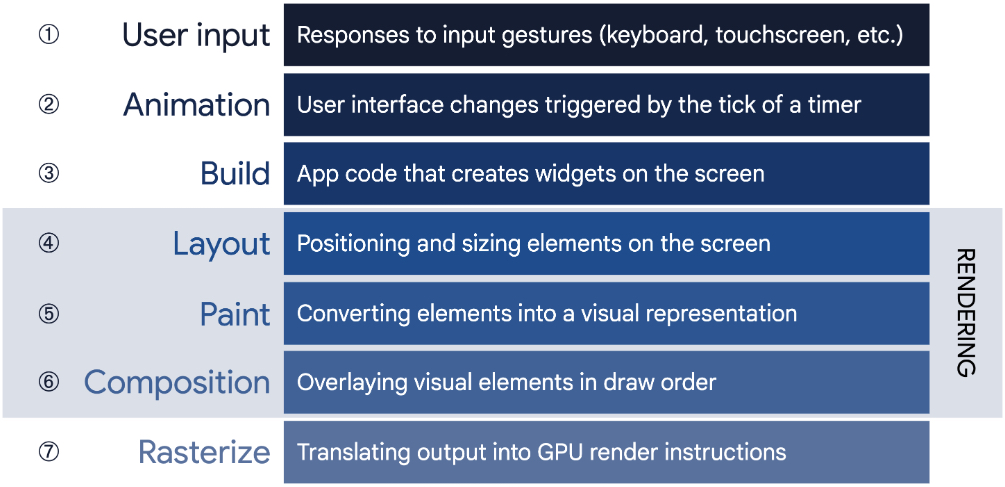
\includegraphics[width=\textwidth]{img/flutter_render_pipeline}
    \caption{Flutter rendering flow (Source: \cite{flutter_docs_architecture})}
    \label{fig:flutter_render_flow}
\end{figure}

Figure \ref{fig:flutter_render_flow} shows Flutter's rendering flow. Flutter is a "reactive, pseudo-declarative UI framework" which means the app's state and user interface layout are separate. User input affects the state, which then results in UI rebuild. Flutter solution to this methodology is the existence of three interconnected trees: \emph{Widget Tree}, \emph{Element Tree}, and \emph{Render Tree} (see Figure \ref{fig:flutter_trees}). The primary components of the framework are widgets which are combined to create user interfaces. For each widget in the tree, the element object is created, and for each element- a render object. The element acts as a connector between widgets and their render objects. Whenever the app's state changes, runtime types of widgets and render objects are checked. Only if they are different, a new render object needs to be created. Otherwise, it is simply updated which is "cheap" performance-wise, just as rebuilding widgets thanks to the fact they are immutable \cite{flutter_docs_architecture}.

\begin{figure}[h]
    \centering
    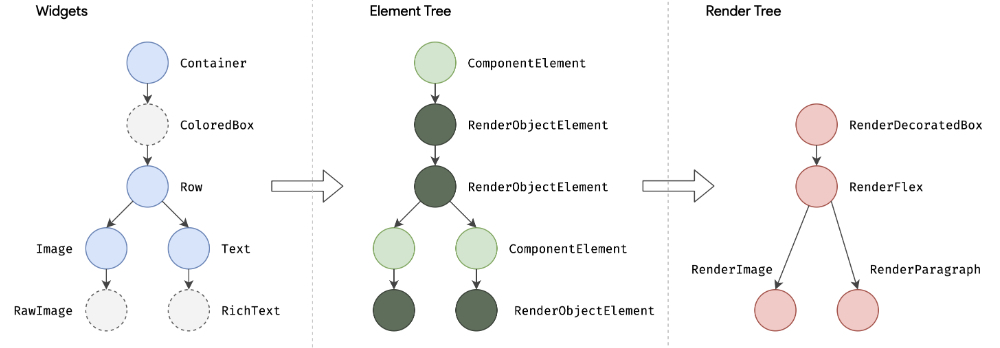
\includegraphics[width=\textwidth]{img/flutter_trees}
    \caption{Flutter Widget, Element, Render trees (Source: \cite{flutter_docs_architecture})}
    \label{fig:flutter_trees}
\end{figure}

\subsubsection*{User interface design}

By default, when creating a new Flutter project, the application depends on the Material library resulting with an appearance mostly found on Android devices, in compliance with the design system described in chapter \ref{chap:android}. Even though it is possible to build such an application for any supported operating system, in most cases a different UI should be preferred for iOS devices to guarantee accordance with Human Interface Guidelines as well as platform styling conventions, as described in chapter \ref{chap:ios}. The components for iOS system are contained in the Cupertino library. Therefore, it is necessary to decide on a design approach early on. Should it be required for the application to have the exact same looks on all platforms (Material, Cupertino or custom), a single UI codebase is an obvious solution. However, if the appearance should be completely platform-specific, there would need to be a separation created and all the layouts would have to be developed in parallel. The third method assumes the usage of the same primary layout components with some minor OS-specific additions, e.g. popups, which does not require the full separation but rather sporadic one. Figures \ref{fig:flutter_material_dialog} and \ref{fig:flutter_cupertino_dialog} show the difference between Material and Cupertino dialogs \cite{flutter_docs_architecture,kosinski_flutter_vs_rn_vs_qt}.

\begin{figure}[h]
    \begin{minipage}{.45\textwidth}
        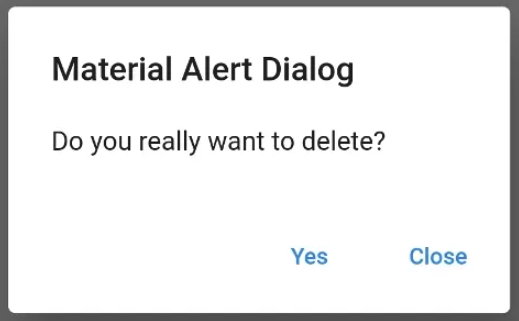
\includegraphics[width=\textwidth]{img/flutter_material_dialog}
        \caption{Flutter Material dialog (Source: \cite{flutter_campus_dialog})}
        \label{fig:flutter_material_dialog}
    \end{minipage}
    \hfill
    \begin{minipage}{.45\textwidth}
        
\includegraphics[width=\textwidth]{img/flutter_cupertino_dialog}
        \caption{Flutter Cupertino dialog (Source: \cite{flutter_campus_dialog})}
        \label{fig:flutter_cupertino_dialog}
    \end{minipage}
\end{figure}

\subsection{React Native}

React Native is a cross-platform framework released in 2015 belonging to the interpreted approach described above. Although, after recent architecture changes, it differs moderately from other solutions of the same type. It is a mobile-only cross-platform framework, meaning that it enables the usage of single codebase for different operating systems, however it is restricted to mobile platforms (Android and iOS). React Native utilizes JavaScript for both application development through React framework and native features access. It is one of the most popular mobile technologies used in the market by some of the biggest companies, e.g. Meta (Facebook), Microsoft (Office, Outlook, Teams), Discord, Tesla, Pinterest, and many more \cite{react_native_showcase, react_native_docs_core_concepts}.

\subsubsection*{Architecture}

\begin{figure}[h]
    \centering
    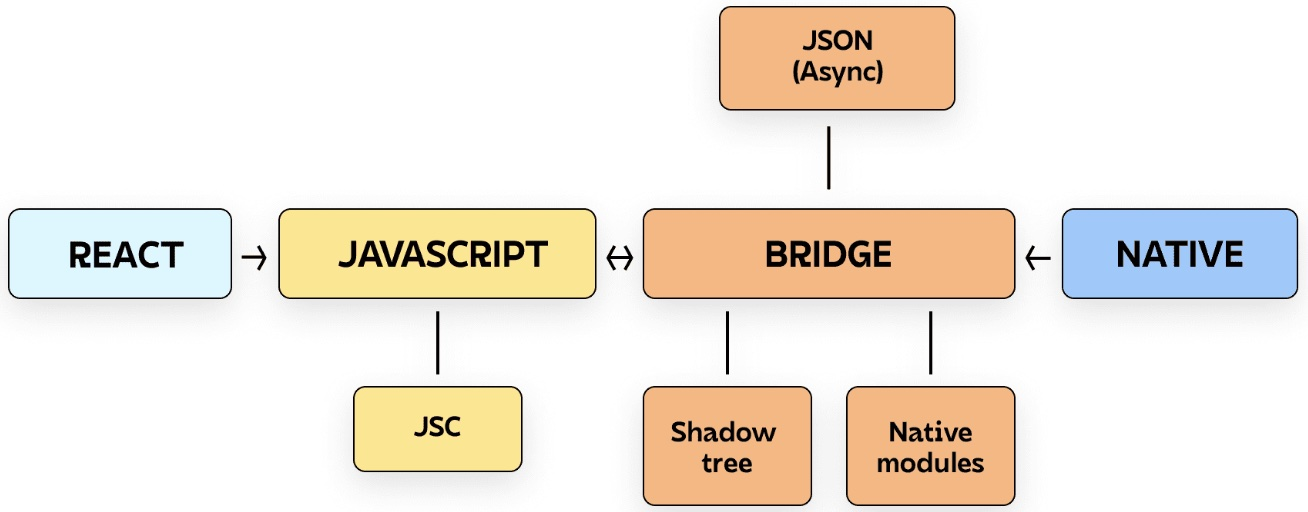
\includegraphics[width=.77\textwidth]{img/rn_old_architecture}
    \caption{React Native previous achitecture (pre-v0.68) (Source: \cite{matijevic_rn_rearchitecture})}
    \label{fig:rn_old_architecture}
\end{figure}

\begin{figure}[h]
    \centering
    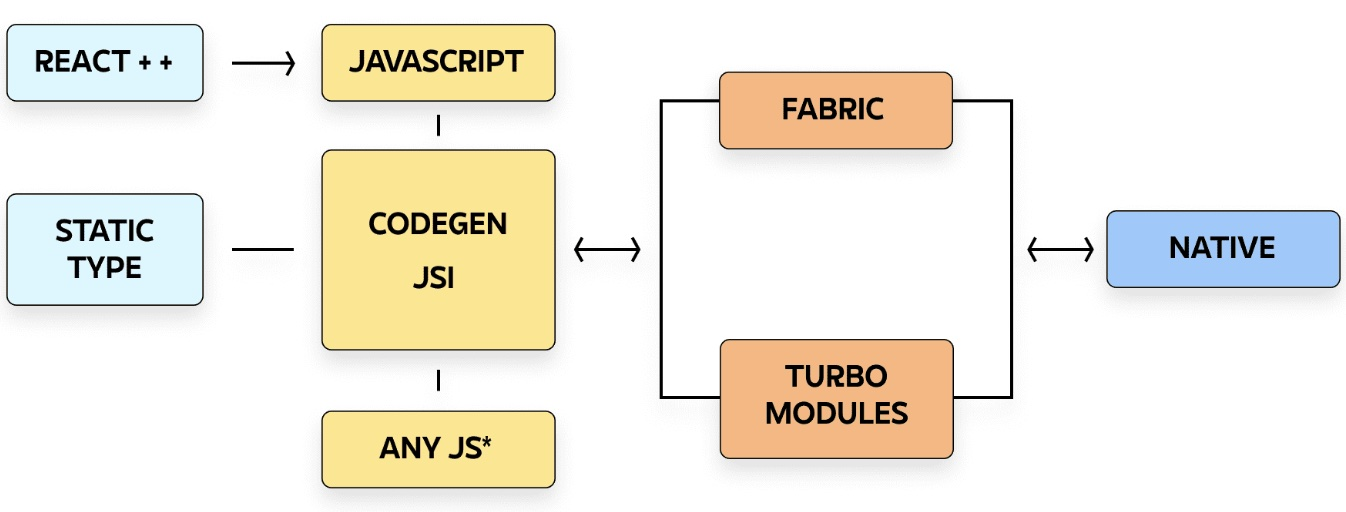
\includegraphics[width=.77\textwidth]{img/rn_new_architecture}
    \caption{React Native New Architecture (v0.68+) (Source: \cite{matijevic_rn_rearchitecture})}
    \label{fig:rn_new_architecture}
\end{figure}

Up until React Native version 0.68 (30 Mar. 2022) the framework's architecture (shown in Figure \ref{fig:rn_old_architecture}) was analogous to the general interpreted cross-platform solution architecture presented in Chapter \ref{chap:cross_platform_approaches}. Because of the drawbacks caused by the \emph{Bridge}, the \emph{New Architecture} (shown in Figure \ref{fig:rn_new_architecture}) has been developed and applied with the release of version 0.68. Table \ref{tab:rn_architecture_improvements} explains the major improvements achieved.

The most important difference is the complete removal of the bridge and bringing the \emph{JavaScript Interface (JSI)} in its place. This change aimed to eliminate the unnecessary delays the bridge caused and the uncertainty of data delivery. Moreover, \emph{JSI} enables the cooperation between Native components and JavaScript via the ability to reference C++ Host objects and call their methods directly \cite{matijevic_rn_rearchitecture}.

\emph{Fabric} is the new React Native's renderer. The rendering process itself is described below. \emph{Fabric} offers many advantages compared to the previous rendering solution. Its core code is shared by target platforms instead of being implemented separately for each of them, thus improving the cross-platform aspect. It decreases the launch time through lazy initialization of native components, as well as enables multithread operations. Overall, there are many benefits guaranteed by Fabric, which together account for the increase in performance and scalability \cite{react_native_docs_fabric}.

\emph{Turbo Modules} are the improved version of \emph{Native Modules}, which were previously the solution to interconnectivity between JavaScript and the native code in order to allow the usage of platform-specific APIs not available directly via JS. \emph{Turbo Modules} take advantage of lazy initialization, thus vastly shortening the loading times \cite{react_native_docs_turbo_modules}.

\emph{Codegen} is an optional helper that assures the validity of the connection between JS and native threads. It automatically (upon the application build) generates the interface files for \emph{Turbo Modules} and \emph{Fabric Native Components}. For \emph{Turbo Modules}, the interfaces provide the \emph{JSI} initializer and functions directly executable from both JS and native sides. For \emph{Fabric Native Components}, the interfaces enable the correct component load at runtime. \emph{Codegen} can be additionally executed by hand when needed \cite{react_native_docs_codegen}.

\begin{table}[h]
    \centering
    \caption{React Native architecture improvements (Source: Own work based on \cite{react_native_docs_why_new_architecture})}
    \label{tab:rn_architecture_improvements}
    \begin{tabular}{ |p{.47\textwidth}|p{.47\textwidth}| }
        \hline
        \multicolumn{1}{|c|}{\textbf{Old architecture}}&\multicolumn{1}{|c|}{\textbf{New Architecture}}\\
        \hline
        \begin{itemize}[nosep]
            \item unnecessary asynchronous wait for processing caused delay 
            \item all the computation was forced to be performed on a single thread
            \item data serialization and deserialization between layers caused additional delays
        \end{itemize}&
        \begin{itemize}[nosep]
            \item synchronous function calls became possible
            \item multithreaded execution is enabled
            \item removed the need to serialize data
            \item new core renderer became shared between platforms
        \end{itemize}\\
        \hline
    \end{tabular}
\end{table}

\subsubsection*{Web support}

As stated before, React Native only allows the development for mobile operating systems. Nevertheless, it is possible to add the support for web with little effort via plugins. The most common solution is \emph{React Native for Web}. It functions as a ``compatibility layer between React DOM and React Native'' \cite{react_native_web_docs}. For example, the general \mintinline{html}{<View>} component used in React Native will be translated to \mintinline{html}{<div>} when building for web, similarly to the conversion performed by React Native itself for mobile platform \cite{harsh_complete_guide_to_rn_web}. 

\subsubsection*{Rendering}

React Native utilizes a three-phase render pipeline. The process flow is presented in Figure \ref{fig:rn_render_flow}. The phases are: \emph{Render}, \emph{Commit} and \emph{Mount}. The \emph{Render} phase constitutes of creation of \emph{React Element Trees} and \emph{React Shadow Trees}. The \emph{Commit} phase is responsible for determining which trees are ready to proceed to the final step, as well as calculating the layout constraints. In the \emph{Mount} phase, the \emph{Host View Tree} is build based on the finalized \emph{React Shadow Tree} \cite{react_native_docs_render}.

The tree creation process is similar to the one applied in the Flutter framework. In React Native, the building blocks of user interface layouts are \emph{React Elements} written in JavaScript. Each of them is translated to a single \emph{React Host Component} which is able to become transformed into a platform-specific equivalent, e.g. \mintinline{html}{<Text>} can become \mintinline{html}{<TextView>} for Android. Those components connected together form a \emph{React Element Tree}. Subsequently, each \emph{React Host Component} is a base for a \emph{React Shadow Node} which offers additional information: props and layout constraints (position and size). Finally, a \emph{Host View Tree} is created, where each node (\emph{Host View}) is rendered on the screen using the corresponding platform-specific component set up according to the properties and constraints obtained. Figure \ref{fig:rn_trees} illustrates the  example of a tree creation process for a simple layout consisting of only text (built for Android). \cite{react_native_docs_render}.

\begin{figure}[h]
    \centering
    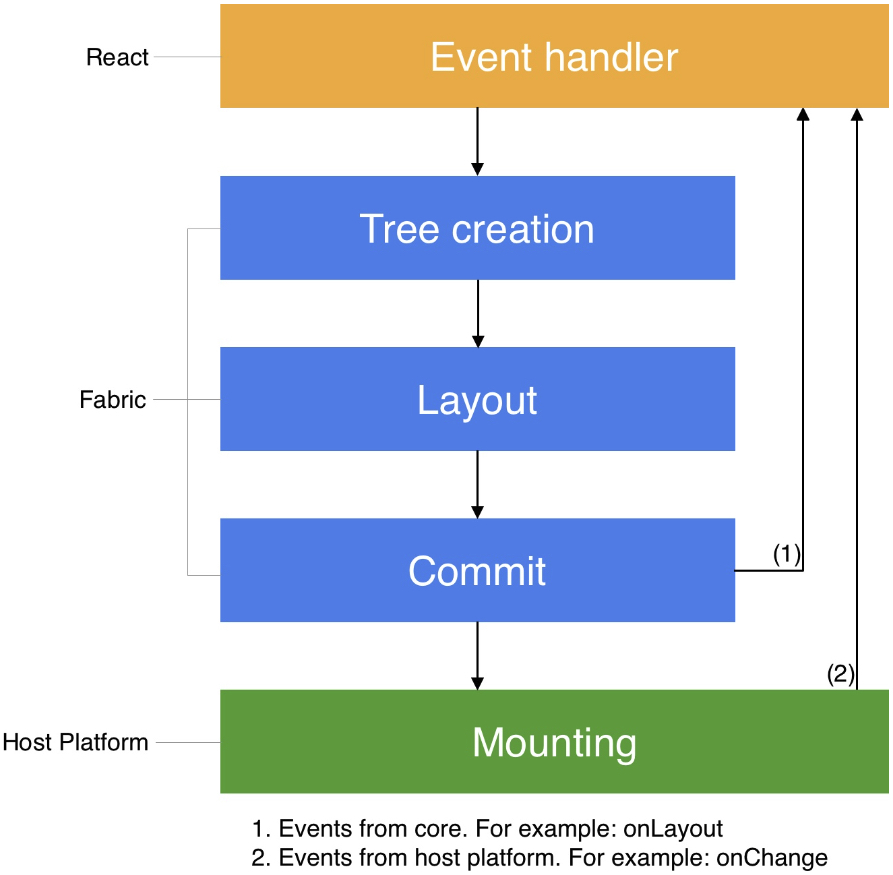
\includegraphics[width=.55\textwidth]{img/rn_render}
    \caption{React Native rendering flow (Source: \cite{react_native_docs_render})}
    \label{fig:rn_render_flow}
\end{figure}

\begin{figure}[h]
    \centering
    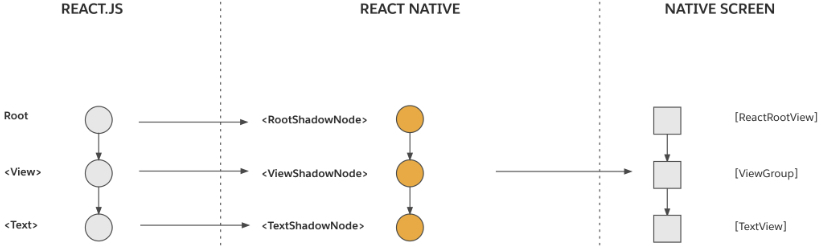
\includegraphics[width=\textwidth]{img/rn_trees}
    \caption{React Native React Element, React Shadow, Host View trees (Source: \cite{react_native_docs_render})}
    \label{fig:rn_trees}
\end{figure}

The complete rendering process takes place across three threads: \emph{UI}, \emph{JS}, and \emph{Background}. The first is responsible for host view management, the second facilitates the render phase and the third handles layouts. A \emph{View Flattening} algorithm is leveraged with the goal of reducing the depth of layout trees whenever possible.  \cite{react_native_docs_render,react_native_docs_view_flattening,react_native_docs_threading}. 

\subsubsection*{User interface design}

As explained in the Rendering section, React Native's user interface components end up being converted into platform native components. Therefore, in the context of UI design and user experience level, it is on par with the native development itself. This remains true even when extending the application to support web, although in this case some limitations may arise as not all the React Native components have their web component equivalent, e.g. when needing to access mobile platform native features \cite{harsh_complete_guide_to_rn_web}.

\subsection{Ionic}

Ionic is a cross-platform mobile framework belonging to the hybrid approach explained above. It enables building Android and iOS apps as well as Progressive Web Apps. It is the oldest out of the three solutions described in this chapter, with its initial release being in 2013. Ionic is platform-agnostic, therefore the app itself can be implemented with a variety of web technologies, e.g. HTML+CSS+JS, React, Angular or Vue. Some of the more popular apps built with Ionic are Sanvello, Sworkit, National Health Service and Instant Pot \cite{ionic_customers,ionic_docs_overview}.

\subsubsection*{Architecture}

\begin{figure}[h]
    \centering
    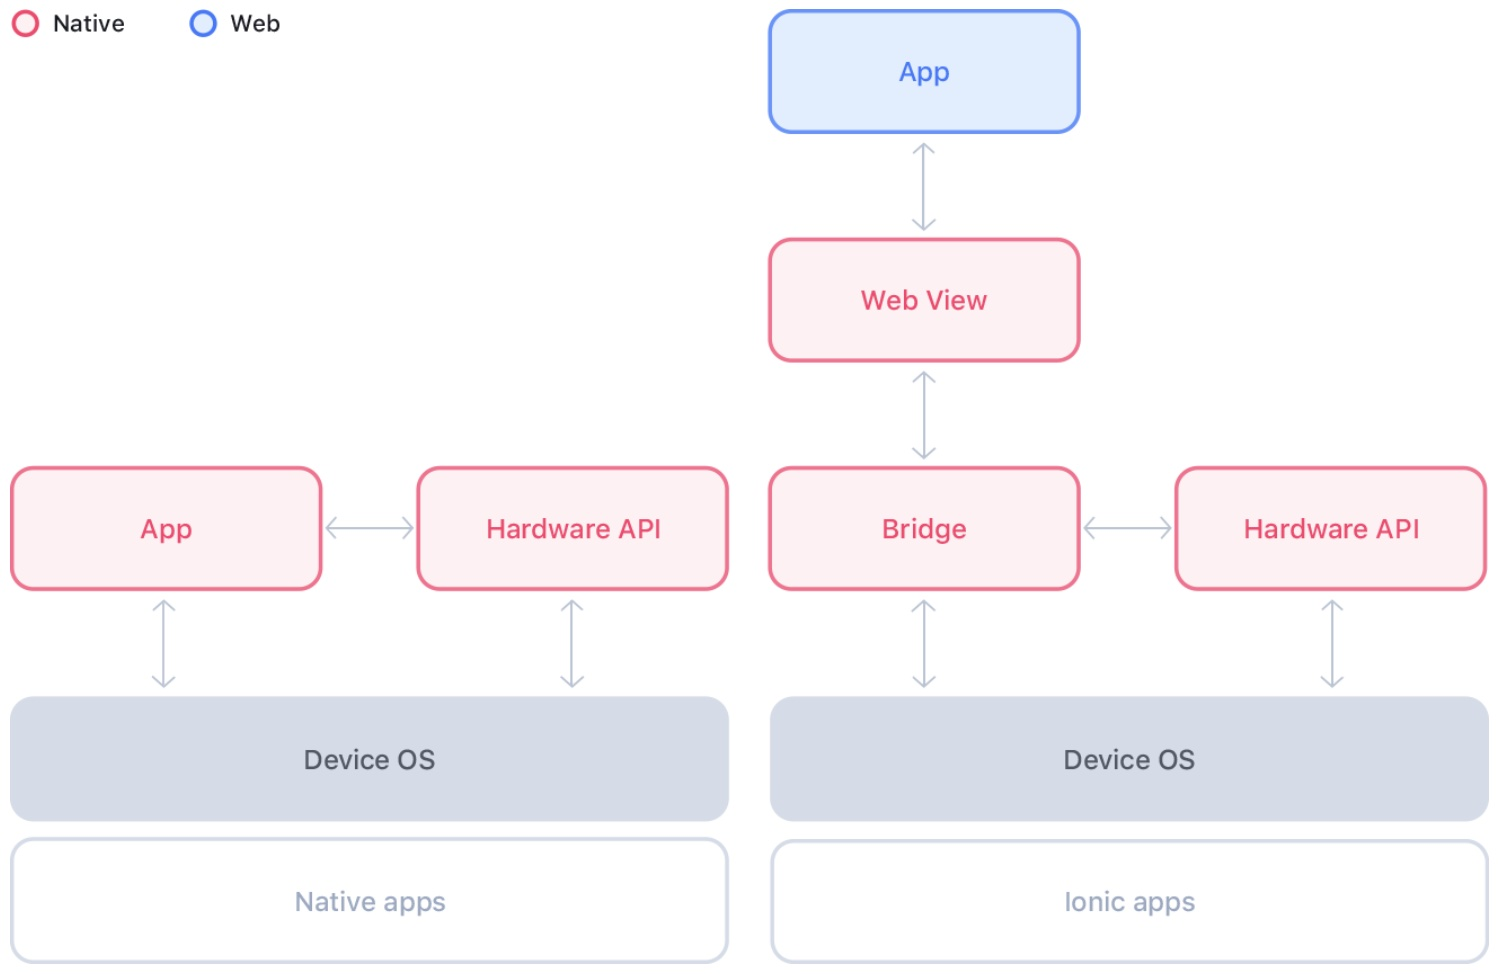
\includegraphics[width=\textwidth]{img/ionic_architecture}
    \caption{Ionic (right) vs native (left) architecture (Source: \cite{ionic_docs_architecture})}
    \label{fig:ionic_architecture}
\end{figure}

The high-level model of an Ionic app architecture is presented in Figure \ref{fig:ionic_architecture} with a side-to-side comparison to a truly native app architecture. As can be expected in the case of a hybrid cross-platform framework, the additional components are: \emph{Web View} and \emph{Bridge}. The development results in a web app which runs inside a \emph{Web View}. Communication between the app and the target platform is facilitated by messaging across the \emph{Native Bridge} and \emph{Native Runtime}. Ionic is simply a UI toolkit for cross-platform app creation, meaning it provides tools for user interface development. On the other hand, \emph{Capacitor} is the primary solution combined with Ionic to provide the possibility of multi-target deployment through providing the above-mentioned \emph{Native Bridge} and \emph{Native Runtime}.
The former utilizes a \emph{runtime JS API} and is responsible for providing an interface for plugins and native methods, as well as passing the messages. The latter handles plugin initialization and executes requested native methods in an asynchronous manner \cite{capacitor_how_works,ionic_docs_architecture,ionic_web_native}.

\subsubsection*{Web support}

Ionic allows to deploy the application as a Progressive Web App and native apps in parallel based on the single codebase. No architectural changes are required for such a use-case, as it is enabled by \emph{Capacitor} itself \cite{ionic_docs_pwa}.

\subsubsection*{Rendering}

Ionic utilizes web technologies, therefore the rendering process is dependent on the choice of such technology. For the sake of this thesis only Ionic with React will be considered, thus the Ionic's rendering process will be simply the React's rendering process.

\begin{figure}[h]
    \centering
    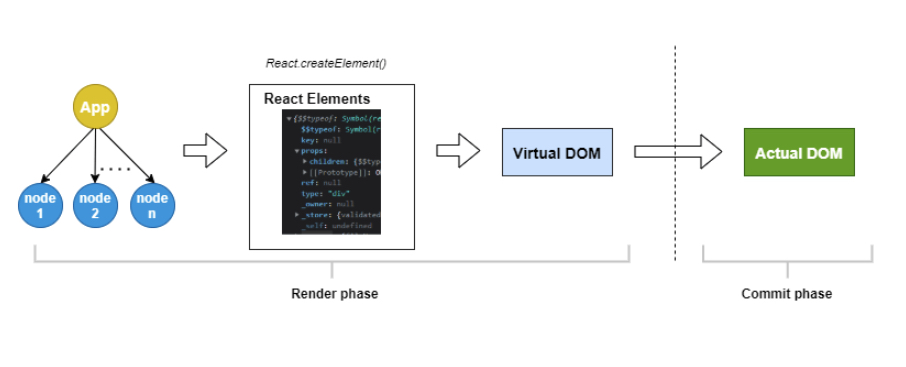
\includegraphics[width=\textwidth]{img/react_render}
    \caption{React rendering flow (Source: \cite{imoh_react_rendering})}
    \label{fig:react_render}
\end{figure}

React rendering pipeline consists of two phases: \emph{Render} and \emph{Commit} (see Figure \ref{fig:react_render}). The former constitues of \emph{JSX} code being used to create the \emph{React Element Tree} which is a \emph{JS} representation of HTML Document Object Model (DOM). In the case of view updating, the elements which have been affected by changes are marked. DOM manipulation is a costly operation, therefore React creates a virtual DOM and only rebuilds parts of the real DOM which need to be updated. The algorithm used to claculate the most efficient re-render is the \emph{Diffing Algorithm}. In the \emph{Commit} phase, the actual DOM is updated based on the previous phase outcomes \cite{imoh_react_rendering}.

\subsubsection*{User interface design}

Being a hybrid framework, Ionic does not use native layout components when rendering the user interface. Instead, Ionic offers configurable components which are visually similar to their native equivalents. Furthermore, they are adaptive to the platform. For Android and web, Material Design is imitated and for iOS, the native controls are mimicked as well. The potential issue to consider is the fact that Ionic only supports Material Design 2, while Material Design 3, or Material You, has been released in 2021 and many tools have already adapted to it. When combining Ionic with Capacitor, it becomes possible to build layouts using native components, however they will still be inside the web view, rather than embedded into the view hierarchy \cite{ionic_docs_core_concepts,ionic_blog_capacitor}.

\subsection{Comparison}

The following Table \ref{tab:framework_comparison} includes the summarized comparison between Flutter, React Native and Ionic.

\begin{table}[ht]
    \centering
    \caption{Cross-platform framework comparison (Source: Own work)}
    \label{tab:framework_comparison}
    \begin{tabular}{ |l| >{\centering}p{35mm}| >{\centering}p{35mm}| >{\centering\arraybackslash}p{35mm}| }
        \hline
        \multicolumn{1}{|c|}{\textbf{Characteristic}}&\textbf{Flutter}&\textbf{React Native}&\textbf{Ionic}\\
        \hline
        Type&Cross-compiled&Interpreted&Hybrid\\
        \hline
        Initial release&2017&2015&2013\\
        \hline
        Current version&3.10&0.71&7.0\\
        \hline
        Platforms&
        \begin{itemize}[nosep]
            \item Android
            \item iOS
            \item Web
            \item Windows
            \item macOS
            \item Linux
        \end{itemize}&
        \begin{itemize}[nosep]
            \item Android
            \item iOS
            \item Web (requires a plugin)
        \end{itemize}&
        \begin{itemize}[nosep]
            \item Android
            \item iOS
            \item Web
            \item Windows (with Electron)
            \item macOS (with Electron)
        \end{itemize}\\
        \hline
        Technology&Dart&React&Any web technology\\
        \hline
        Rendering&Canvas drawing&Native components&Web View wrapper\\
        \hline
        Native APIs&Direct access&Direct access&Indirect access\\
        \hline
    \end{tabular}
\end{table}

\subsection{Evaluation of cross-platform frameworks}\label{chap:eval_cross_platform}

Considering the ongoing changes to the mobile market as well as the saturation of different cross-platform solutions, performing the selection of a specific framework for application development becomes a more and more complicated task. Especially because for each use-case there might be a different optimal solution based on different aspects such as business costs, development limitations, etc. For that reason, a few evaluation methods have been proposed in the literature, some of them very simple and some of them more detailed. There is a lot of scientific work performing the assessment of a selection of available cross-platform frameworks according to those methods. The issue with such evaluation outcome lays in the fact it can become out-dated in a short time with the breaking updates to the considered technologies. For example, a majority of literature on the topic of cross-platform development considers a tool Adobe PhoneGap which has been discontinued and thus is no longer relevant. Therefore, the assessment frameworks themselves are a strong base for performing further research  without the risk of becoming obsolete, while the actual assessment ought to be repeated over time to ensure up-to-date results.

\begin{table}[h]
    \centering
    \caption{Cross-platform framework evaluation criteria (Source: Own work based on \cite{rieger_eval_cp})}
    \label{tab:eval_criteria}
    \begin{tabular}{ |l|p{.78\textwidth}| }
        \hline
        \textbf{Perspective}&\textbf{Criteria}\\
        \hline
        Infrastructure&License, Supported target platforms, Supported development platforms, Distribution channels, Monetization, Internationalization, Long-term feasibility\\
        \hline
        Development&Development environment, Preparation time, Scalability, Development process fit, User interface design, Testing, Continuous delivery, Configuration management, Maintainability, Extensibility, Integrating custom code, Pace of development\\
        \hline
        App&Access to device-specific hardware, Access to platform-specific functionality, Support for connected devices, Input device heterogeneity, Output device heterogeneity, Application life cycle, System integration, Security, Robustness, Degree of mobility \\
        \hline
        Usage&Look and feel, Performance, Usage patterns, User authentication\\
        \hline
    \end{tabular}
\end{table}

Table \ref{tab:eval_criteria} provides an overview of some of the evaluation criteria proposed in the literature, divided into four perspectives: Infrastructure, Development, App and Usage. The first perspective revolves around licensing, platform support, distribution and long-held operability. Development perspective considers all the aspects directly connected to software development, e.g. available IDEs, learning and implementation effort, scalability, user interface design abilities, maintainability and testing. App perspective includes mainly security, hardware access and external devices. Finally, Usage perspective concerns the aspects connected with end-user experience such as app appearance and behavior, authentication and performance \cite{eval_rn_flutter,rieger_eval_cp}.

The process of the complete evaluation of a single cross-platform framework according to the above-mentioned criteria is a complex and labor-consuming task perfectly fitting into the methodology of Multi-Criteria Decision-Making (MCDM). This methodology can provide a standardized way of approaching the issue of framework selection. Some of the popular solutions for MCDM are Analytic Hierarchy Process (AHP), Technique for Order of Preference by Similarity to Ideal Solution (TOPSIS) or Multi-attribute Utility Theory (MAUT). In the literature there are also proposed approaches created from the merge of a subset of those solutions, e.g. Integrated Multi-Criteria Decision-Making \cite{lachgar_mcdm_cp}.
